\chapter{PROJETO DO BANCO DE DADOS}

\section{Modelo de dados e relacionamentos}

O banco de dados foi projetado a partir das informações necessárias aos processos descritos no Capítulo 2, partindo do modelo conceitual para o lógico \cite{elmasri2019}. Optou-se pelo modelo relacional no Microsoft SQL Server porque as operações do sistema são transacionais e envolvem várias tabelas ao mesmo tempo: a saída de um veículo, por exemplo, altera o carregamento, o veículo, os pedidos e cada caixa, além de gerar o registro de portaria e as movimentações. Essas alterações precisam ser confirmadas ou desfeitas em conjunto, garantia oferecida pelas propriedades ACID \cite{silberschatz2020}.

A Figura~\ref{fig:er} apresenta o modelo entidade-relacionamento, em notação de Chen, com as doze entidades centrais e suas cardinalidades. O relacionamento \textit{Leva}, entre carregamento e pedido, tem atributos próprios (resultado e motivo da entrega) e, por isso, torna-se a tabela associativa \texttt{CarregamentoPedidos} no modelo lógico. A movimentação de caixa foi modelada como entidade fraca, pois só existe vinculada a uma caixa.

\begin{sidewaysfigure}
\centering
\caption{Modelo entidade-relacionamento (notação de Chen)}
\label{fig:er}
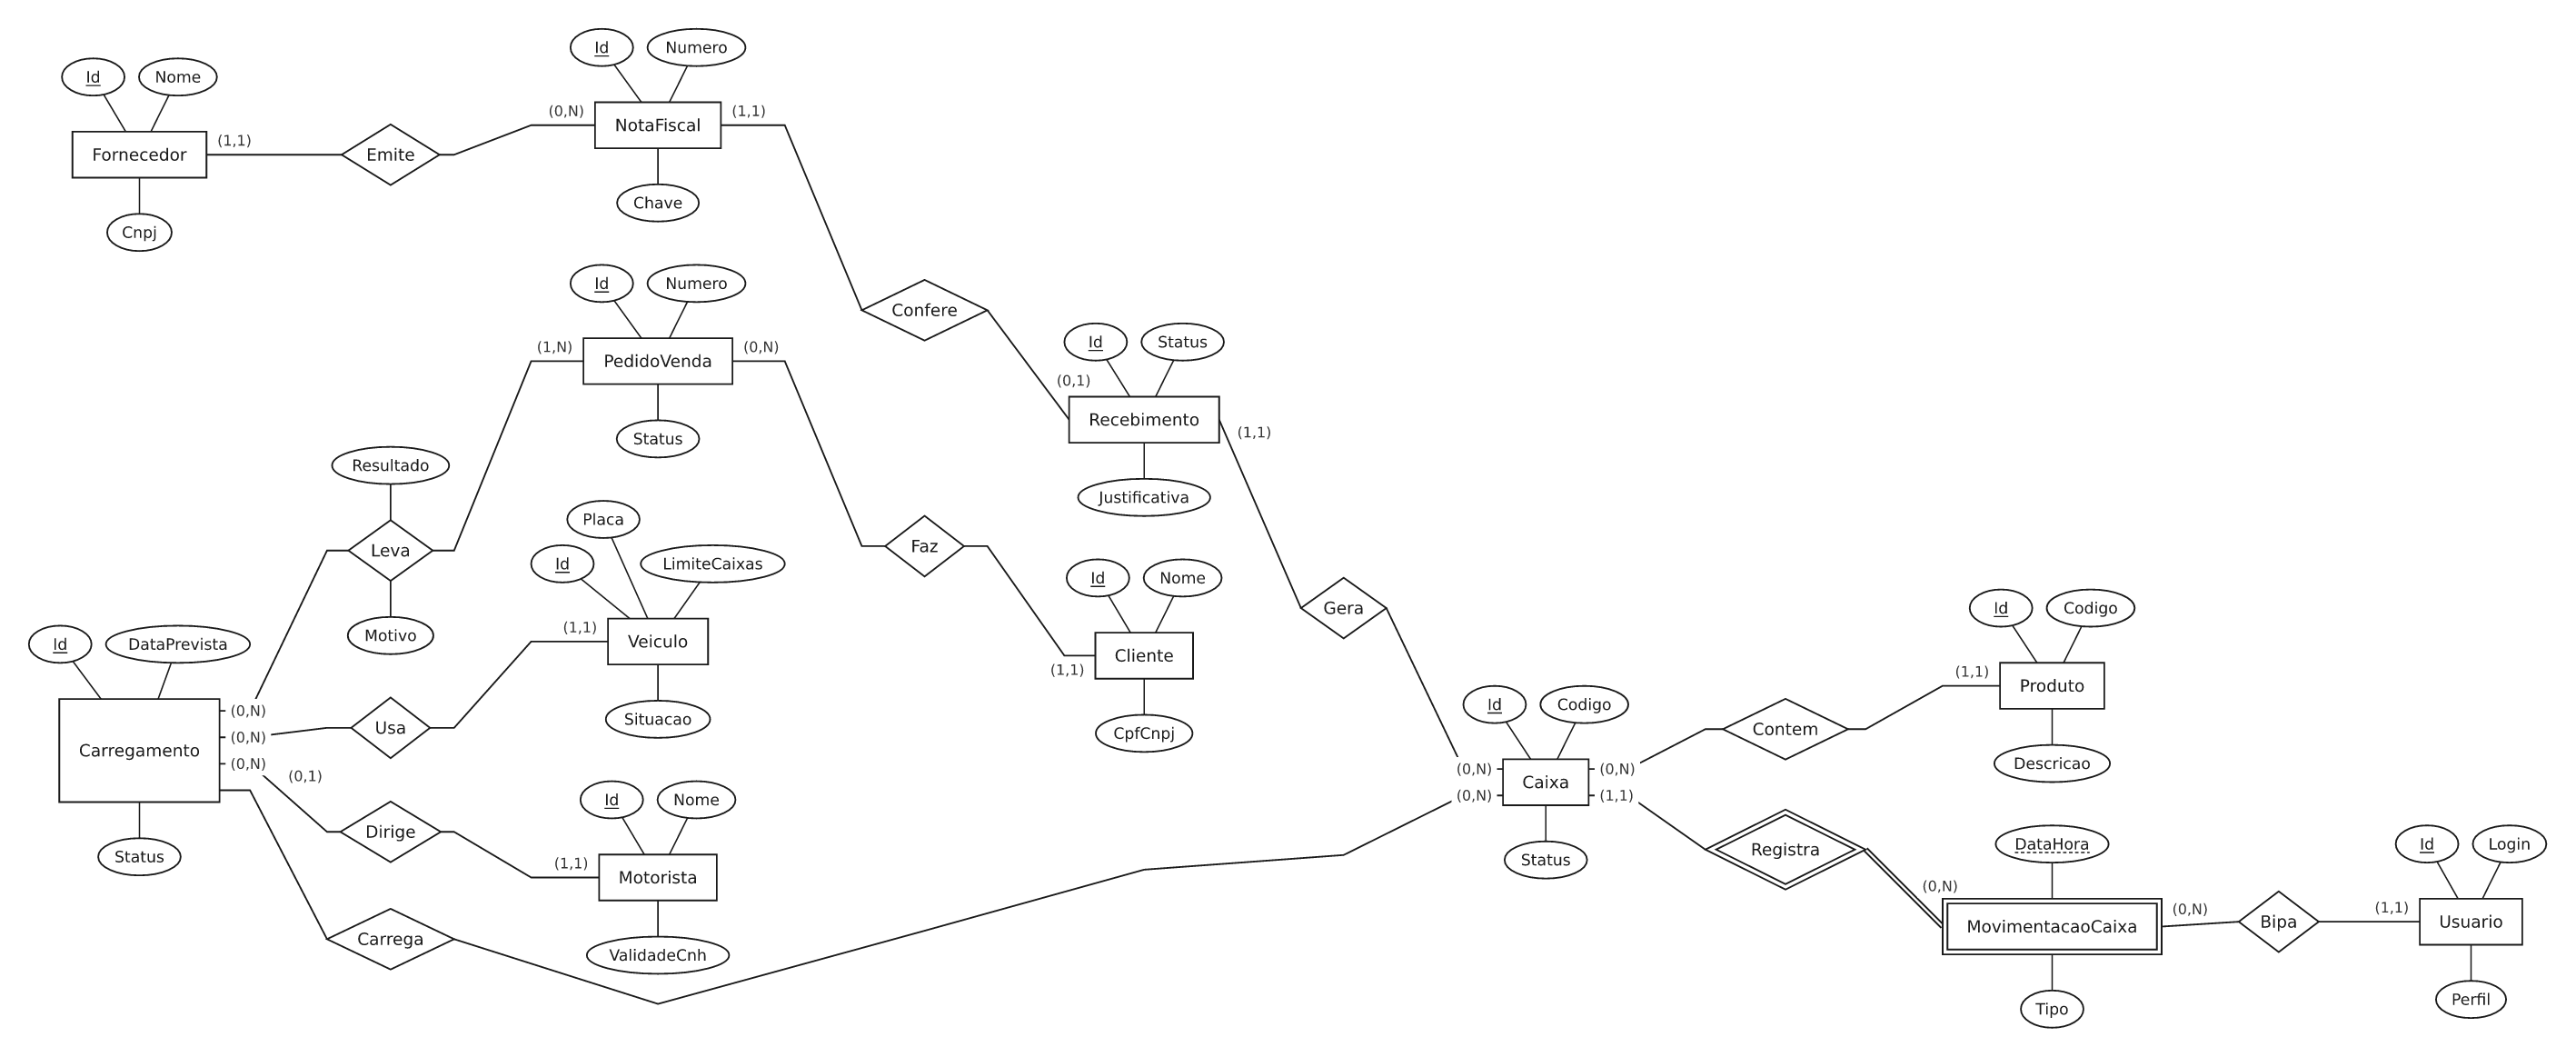
\includegraphics[width=24cm]{figuras/er.png}
\fonte{Elaborado pelo autor (2026)}
\end{sidewaysfigure}

O modelo lógico tem dezenove tabelas, criadas pelo Entity Framework Core a partir das classes C\# por meio de \textit{migrations}. A Tabela~\ref{tab:tabelas} agrupa as tabelas pela origem dos dados.

\begin{table}[htbp]
\centering
\caption{Principais tabelas do banco de dados}
\label{tab:tabelas}
\footnotesize
\begin{tabular}{|p{2.6cm}|p{6.2cm}|p{5.6cm}|}
\hline
\textbf{Grupo} & \textbf{Tabelas} & \textbf{Finalidade} \\ \hline
Vindas do ERP & Clientes, Enderecos, Fornecedores, Produtos, PedidosCompra, NotasFiscais, PedidosVenda e seus itens & Cópia dos dados mestres e dos pedidos; o sistema só altera o status do pedido \\ \hline
Acesso & Usuarios & Login, \textit{hash} da senha e perfil \\ \hline
Entrada & Recebimentos, Caixas, MovimentacoesCaixa & Conferência, etiqueta única de cada caixa e histórico de cada leitura \\ \hline
Frota & Veiculos, Motoristas & Situação do veículo, limite de caixas e validade da CNH \\ \hline
Expedição & Carregamentos, CarregamentoPedidos, RegistrosPortaria & Viagens, resultado das entregas e passagens pela portaria \\ \hline
\end{tabular}
\fonte{Elaborado pelo autor (2026)}
\end{table}

\section{Procedures e triggers}

Duas regras foram reforçadas no próprio banco por \textit{triggers}, para valerem mesmo diante de um comando SQL executado fora da aplicação. A primeira impede o cadastro de carregamento com veículo em manutenção (RN17). A segunda impede apagar o histórico de movimentação das caixas, preservando a rastreabilidade, como mostra o código a seguir.

\begin{codeblock}[Trigger que protege o histórico das caixas]{SQL}
CREATE TRIGGER TR_MovimentacoesCaixa_ImpedeExclusao
ON MovimentacoesCaixa
INSTEAD OF DELETE
AS
BEGIN
    THROW 50002, 'O historico de movimentacao das caixas nao pode ser apagado.', 1;
END
\end{codeblock}

Também foram criadas duas \textit{procedures}: \texttt{sp\_HistoricoCaixa}, que devolve todas as movimentações de uma caixa a partir do código da etiqueta (RF19), com produto, tipo, horário, usuário e carregamento; e \texttt{sp\_ResumoCarregamento}, que compara o total de caixas dos pedidos de um carregamento com as caixas já bipadas, base da regra de liberação da saída (RN11). Todos esses objetos são criados por \textit{migration} e, portanto, ficam versionados junto com o código.

\section{Estratégias de otimização}

As consultas mais frequentes são buscas pontuais disparadas pelas leituras de código: caixa pelo código da etiqueta, nota pela chave, veículo pelo identificador do QR Code e usuário pelo login. Para essas colunas foram criados índices únicos, que garantem a regra de unicidade e transformam a busca em acesso direto, sem varredura da tabela; o mesmo vale para placa, CPF do motorista e número do pedido. As chaves estrangeiras recebem índices automaticamente, o que acelera as junções entre carregamento, pedidos e caixas. Os campos de texto indexados têm tamanho máximo definido, e os status são gravados como inteiros. As consultas usadas nas telas carregam de uma só vez os dados relacionados de que precisam, evitando múltiplas idas ao banco por registro.

\section{Mecanismos de segurança}

A segurança do banco combina medidas de integridade e de proteção de dados. As senhas são armazenadas apenas como \textit{hash} BCrypt, nunca em texto. Nenhuma chave estrangeira apaga dados em cascata, de modo que nenhum registro histórico é removido indiretamente, e o \textit{trigger} apresentado bloqueia a exclusão das movimentações. A aplicação acessa o banco somente pelo Entity Framework, com comandos parametrizados, o que evita injeção de SQL. Para a implantação em produção, prevê-se um usuário de banco com privilégios mínimos para a aplicação, conexão criptografada com TLS e cópias de segurança automáticas do serviço de nuvem, além da retenção limitada dos dados pessoais, conforme a LGPD \cite{brasil2018lgpd}.
